\documentclass[a4paper, 12pt]{article}
\usepackage[T2A]{fontenc}
\usepackage[left=2cm,right=2cm,top=2cm,bottom=2cm]{geometry}
\usepackage[russian]{babel}
\usepackage{amsfonts,amsmath,amssymb}
\usepackage{mathrsfs}
\usepackage{graphicx}
\usepackage{color}
\usepackage[normalem]{ulem}
\usepackage{wrapfig}
\usepackage{fancyhdr}
\usepackage{floatflt}
\usepackage{python}
\usepackage{indentfirst}
\usepackage{setspace}
\usepackage{scrextend}
\usepackage{listings}
\usepackage{makecell,tabularx}

\definecolor{grey}{RGB}{40, 40, 40}

\lstdefinestyle{CommentStyle}{
    language=XML,
    %numbers=left, numberstyle=\tiny, stepnumber=1, numbersep=5pt,
    commentstyle=\color{red},
	basicstyle=\footnotesize\ttfamily,
	language={[ANSI]C++},
	keywordstyle=\bfseries,
	showstringspaces=false,
	morekeywords={include, printf},
	commentstyle={},
	escapeinside=§§,
	escapebegin=\begin{russian}\commentfont,
	escapeend=\end{russian},
    keywordstyle=\color{blue}\bfseries,
    morekeywords={align,begin},
    extendedchars=\true,
    tabsize=2
}
\lstdefinestyle{myLatexStyle}{
    language=c++,
    %backgroundcolor=\color{grey},
    numbers=left, numberstyle=\tiny, stepnumber=1, numbersep=5pt,
    commentstyle=\color{red},
    keywordstyle=\color{blue}\bfseries,
    morekeywords={align,begin},
    extendedchars=\true,
    tabsize=2
}

\lstdefinestyle{pmyLatexStyle}{
    language=java,
    %backgroundcolor=\color{grey},
    numbers=left, numberstyle=\tiny, stepnumber=1, numbersep=5pt,
    commentstyle=\color{red},
    keywordstyle=\color{blue}\bfseries,
    morekeywords={align,begin},
    extendedchars=\true,
    tabsize=2
}

\setlength{\parindent}{12,5mm}

\onehalfspacing

\pagestyle{fancy}
\renewcommand{\sectionmark}[1]{\markright{#1}}
\fancyhf{} 
\fancyhead[R]{\bfseries\thepage}
\fancyhead[LO]{\bfseries\rightmark}

\newcommand{\image}[3]{
	\begin{figure}[ht]
		\center{\includegraphics[height=#2pt]{img/#1} }
		\caption{\textit{#3}}\end{figure}
}
%\title{Проектная работа по теме:«Персистенция в реальной жизни»}

\newcommand{\cmd}[1]{\immediate\write18{#1}}
\newcommand{\pf}[1]{\immediate\input{#1}}
% \newcommand{\n}{ }
% \newcommand{\py}[1]{
% 	\cmd{
% 		k=''&&py=${k}&&n='exec("""def vip(l,k):\\n    for i in range(len(l)):\\n        try:\\n            if l[i]==";":i,k=i+1,k+("\\\\n")\\n            else: k+=l[i]\\n        except:break\\n    exec(k)\\n""");vip("""#1""".replace("|",chr(32)).replace(";"+chr(32),";"),"")'&&printf ${n// /|}>latex.py
% 		}
% 	\cmd{
% 		python3 latex.py>py.out 2>py.log
% 		}
% 	\pf{
% 		py.out
% 	   }
% 	}

\begin{document}
\thispagestyle{empty}
\begin{floatingfigure}{5.8cm}
	
\includegraphics[width=5.8cm,height=3.5cm,keepaspectratio]{img/logo.png}
	\vspace{0cm}
\end{floatingfigure}

\sloppy{
	\scriptsize{
		\line(6,0){0}

		\centering Департамент образования и науки города Москвы

		\centering ГОСУДАРСТВЕННОЕ БЮДЖЕТНОЕ

		\centering ОБЩЕОБРАЗОВАТЕЛЬНОЕ УЧРЕЖДЕНИЕ ГОРОДА

		\centering МОСКВЫ «КУРЧАТОВСКАЯ ШКОЛА»

		\line(6,0){300}

		\centering 123060, Москва, улица Маршала Конева, дом 10.

		\centering \textbf{Тел: (499) 194-10-44, E-mail: kurchat@edu.mos.ru}

		\line(6,0){0}
	}}

\topskip=-200pt
\vspace*{130px}
\begin{Huge}
	\textbf{\center{Проектная работа по теме:\\«Персистенция в реальной жизни»}}
\end{Huge}
\vspace*{5px}
\begin{footnotesize}
	\center {В проекте был рассмотрен эффект персистенции зрения на примере сложного трехмерного опыта.
		В результате опыта получился один из видов голограмм: светодиодная голограмма.
		В рамках проекта также можно найти объяснение, применение и историю эффекта. }
	\vspace*{200px}
	\begin{flushright}
		Выполнил ученик 10 «А» класса\\
		Плютто Андрей Петрович\\
		Руководитель проекта\\
		учитель физики\\
		Горцакалян Жанна Степановна\\
	\end{flushright}
\end{footnotesize}
\begin{normalsize}
	\begin{center}
		Москва\\
		2021 год
	\end{center}
\end{normalsize}
\newpage
\thispagestyle{fancy}
\renewcommand{\sectionmark}[1]{\markright{#1}}
\fancyhf{}
\fancyhead[R]{\bfseries\thepage}
\fancyhead[LO]{\bfseries Оглавление}
\renewcommand{\contentsname}{Оглавление}
\tableofcontents
\newpage
\pagestyle{fancy}
\renewcommand{\sectionmark}[1]{\markright{#1}}
\fancyhf{}
\fancyhead[R]{\bfseries\thepage}
\fancyhead[LO]{\bfseries\rightmark}

\section{Аннотация}
Работа «Персистенция в реальной жизни» посвящена эффекту 
персистенции зрения, наглядно представленному на примере сложного 
трехмерного, иллюстрирующего этот любопытный феномен, опыта. 
Понятие «персистенция зрения» (от лат. persisto - постоянно 
пребывать, оставаться) иначе можно передать как «инерция зрения», 
многочисленные примеры которой были известны еще древним. Скажем, 
если крутить горящий факел, человеческий мозг будет его 
воспринимать — видеть — как огненный круг вместо ряда 
последовательных положений одного и того же горящего факела, 
ходящего по кругу. По сути, речь идет об иллюзии, значимость 
которой отмечали еще древнеиндийские философы. Они утверждали, 
например, что так называемая «человеческая личность»    - тоже 
всего лишь похожий эффект «инерции умозрения». Иллюзия «личности» 
видится нами как «единая целостность», как факельный круг, только 
потому, что наш умственный взор не силах зафиксировать отдельные 
точки движения человеческой души. На этом широком фоне понимания 
сути данного эффекта интересно было представить конкретную краткую 
историю его научного изучения, а также его объяснение и возможное 
применение. Эти задачи выполнены на современном и технически 
актуальном примере создания одного из видов голограмм: на примере 
POV\footnote{\ POV -- Persistence of vision(персистенция 
зрения)}-голограммы.
\newpage
\section{Введение}
\subsection{Актуальность}
POV эффект мы можем наблюдать в реальной жизни каждый день.
Достаточно навести камеру телефона на электронные часы,
и мы сразу увидим частоту обновления кадров (FPS\footnote{FPS -- Frame-Per-Second(кадров в секунду)}).
То, что мы не видим это невооруженным глазом, объясняет POV эффект.
Поэтому POV является чуть ли не самым используемым эффектом анатомии человека.
\subsection{Проблема}
Потенциал персистенции зрения еще не раскрыт полностью. С помощью POV можно
создавать моментально не только 2D экраны, но и полноценные 3D голограммы.
\subsection{Цель работы}
Раскрыть потенциал POV, создать собственную голограмму из подручных средств.
\subsection{Задачи}
\begin{enumerate}
	\item Объяснить, как работает эффект
	\item Объяснить историю его открытия, историю его применения в физике
	\item Выяснить где эффект используется в наше время
	\item Создать собственную 3D поделку на основе данного эффекта
\end{enumerate}
\newpage
\section{Общие сведения о инерции зрения}
\subsection{Определение}
Персистенция зрения традиционно относится к оптической иллюзии,
которая возникает, когда зрительное восприятие объекта не прекращается
в течение некоторого времени после того, как исходящие от него лучи света
перестали попадать в глаз. Иллюзия также была описана как
"персистенция сетчатки", "персистенция впечатлений", просто "персистенция"
и другие варианты. Согласно этому определению, иллюзия будет такой же
или очень похожей на позитивные остаточные образы.

"Постоянство зрения" может также пониматься как-то же самое,
что и "слияние мерцания", эффект, что зрение, кажется, сохраняется
непрерывно, когда свет, который входит в глаза, прерывается с короткими
и регулярными интервалами.

С момента своего появления термин "персистенция зрения" считается объяснением
восприятия движения в оптических игрушках, таких как фенакистископ и зоотроп,
а позже и в кино. Однако эта теория была оспорена еще до появления кинематографа
в 1895 году. Если " постоянство зрения "объяснить, как" слияние мерцания", то его
можно рассматривать как фактор иллюзии движущихся картинок в кино и связанных с ним
оптических игрушках, но не как ее единственный принцип.

Наиболее важным фактором в этом типе анимации является стробоскопический эффект,
подробно описанный изобретателем Саймоном Стампфером, но это было в значительной
степени проигнорировано теоретиками кино (по крайней мере, за пределами Германии и Австрии).


Ранние описания иллюзии часто объясняли этот эффект исключительно несовершенством
глаз, особенно сетчатки. Нервы и части мозга позже стали частью объяснений.
\subsection{Почему возникает?}

Эффект возникает при переполнении, перенасыщении палочек глаза.
Дело в том, что наш глаз состоит из палочек и колбочек: колбочки отвечают
за различие цветов, а палочки за насыщенность цвета. Когда цвет в
колбочках перенасыщается уже не можем различать один цвет от другого и
видим их все вместе.

\image{глаз.png}{340}{Строение человеческого глаза}

\newpage

\section{История POV}

Первое упоминание о персистенции зрения сделано Аристотелем
в 384-322 годах до н.э. Он первый отметил, что он наблюдает
солнечные лучи еще некоторое время после того как перестает
смотреть на них.

Открытие эффекта часто приписывают римскому поэту Лукрецию
(ок. 15 октября 99 г. до н. э.-ок. 55 г. до н. э.), хотя он лишь упоминает
нечто подобное в связи с образами, увиденными во сне.

Примерно в 165 году нашей эры Птолемей описал в своей книге
"оптика" вращающийся гончарный круг с нанесенными на него
различными цветами. Он отметил, как различные цвета секторов
смешиваются в один цвет и как точки появляются в виде кругов, когда
колесо вращается очень быстро. Когда линии рисуются поперек оси
диска, они заставляют всю поверхность казаться однородной по цвету.

"За зрительным впечатлением, созданным в первом обороте, неизменно
следуют повторные случаи, которые впоследствии производят
тождественное впечатление. Это также происходит в случае падающих
звезд, чей свет кажется расширенным из-за их скорости движения, все
в соответствии с количеством она проходит на ощутимом расстоянии
вместе с чувственным впечатлением, возникающим в зрительной
способности.

Порфирий (около 243-305) в своем комментарии к гармоникам
Птолемея описывает, что чувства не стабильны, а запутанны и неточны.
Определенные интервалы между повторными впечатлениями не
обнаруживаются. Белое или черное пятно на вращающемся конусе (или
вершине) выглядит как круг этого цвета, а линия на вершине
заставляет всю поверхность выглядеть в этом цвете. "Из-за быстроты
движения мы получаем впечатление линии на каждой части конуса,
когда линия движется."

В XI веке Ибн аль-Хайтам, который был знаком с трудами
Птолемея, описал, как цветные линии на волчке не могли быть
различимы как разные цвета, но появлялись как один новый цвет,
состоящий из всех цветов линий. Он сделал вывод, что зрению нужно
некоторое время, чтобы различить цвет. Аль-Хайтам также отметил,
что вершина казалась неподвижной, когда вращалась чрезвычайно
быстро, "поскольку ни одна из ее точек не оставалась неподвижной в
одном и том же месте в течение какого-либо ощутимого времени".

Леонардо да Винчи писал в своей записной книжке: "каждое тело,
которое движется быстро, кажется окрашивающим свой путь
впечатлением своего оттенка. Истинность этого положения видна из
опыта; так, когда молния движется среди темных облаков, скорость ее
извилистого полета делает весь ее путь похожим на светящуюся змею.

Таким же образом, если вы взмахнете зажженным клеймом, весь его
ход будет казаться кольцом пламени. Это происходит потому, что
орган восприятия действует быстрее, чем суждение."

Исаак Ньютон (1642-1726 / 27) якобы продемонстрировал, как
белый свет представляет собой комбинацию различных цветов с
вращающимся диском с цветными сегментами. При быстром вращении
цвета, кажется, смешиваются и кажутся белыми (или, скорее, не
совсем белым светлым оттенком). В его книге 1704 года оптики он
описал машину с призмами, линзой и большой движущейся гребенкой с
зубьями, вызывающими последовательное проецирование
чередующихся цветов. Если это делалось достаточно быстро, то
чередующиеся цвета уже не воспринимались отдельно, а
воспринимались как белые. Ньютон сравнил его принцип с эффектом
следа бенгальского огня: вращающийся горящий уголь может
выглядеть как круг огня, потому что, как он писал: «ощущение угля в
нескольких местах этого круга остается запечатленным на сенсориуме,
пока уголь снова не вернется в то же самое место.»

\image{круг.png}{200}{Ньютоновский опыт с кругом}
В 1768 году Патрик Д'Арси (1725-1779) сообщил, что он измерил
длительность 0,13 секунды для одного полного вращения горящего
угля, в то время как он рассматривался как полный круг света. Он
зарегистрировал несколько вращений специально построенной машины
в своем саду и в сотрудничестве с наблюдателем, который обладал
превосходным зрением (собственное зрение Д'Арси было повреждено в
результате несчастного случая). Д'Арси подозревал, что
продолжительность может отличаться у разных наблюдателей,
интенсивность света вращающихся объектов, цвета и расстояния
наблюдения. Он планировал дальнейшие эксперименты, чтобы
определить такие возможные различия, но, похоже, никаких
результатов опубликовано не было.

Будучи студентом университета, Джозеф Плато заметил в
некоторых своих ранних экспериментах, что при взгляде с небольшого
расстояния на два концентрических зубчатых колеса, которые быстро
вращаются в противоположных направлениях, создается оптическая
иллюзия неподвижного колеса. Позже он прочитал статью Питера
Марка Роже 1824 года и решил исследовать этот феномен дальше. Он
опубликовал свои выводы в Correspondance Mathématique et Physique
\footnote{\ Correspondance Mathématique et Physique -- Математическое и физическое соответствие}
в 1828 году и 1830 году. В 1829 году плато представил свой тогда еще
неназванный анортоскоп в докторской диссертации Sur quelques
propriétés des impressions produites par la lumière sur l'organe de la vue
\footnote{\ Sur quelques
	propriétés des impressions produites par la lumière sur l'organe de la vue --
	некоторых свойствах, производимых светом на зрение}.

\begin{figure}[ht]
	\center{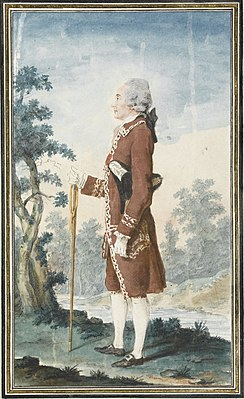
\includegraphics[height=300px]{img/Арси.jpg}
		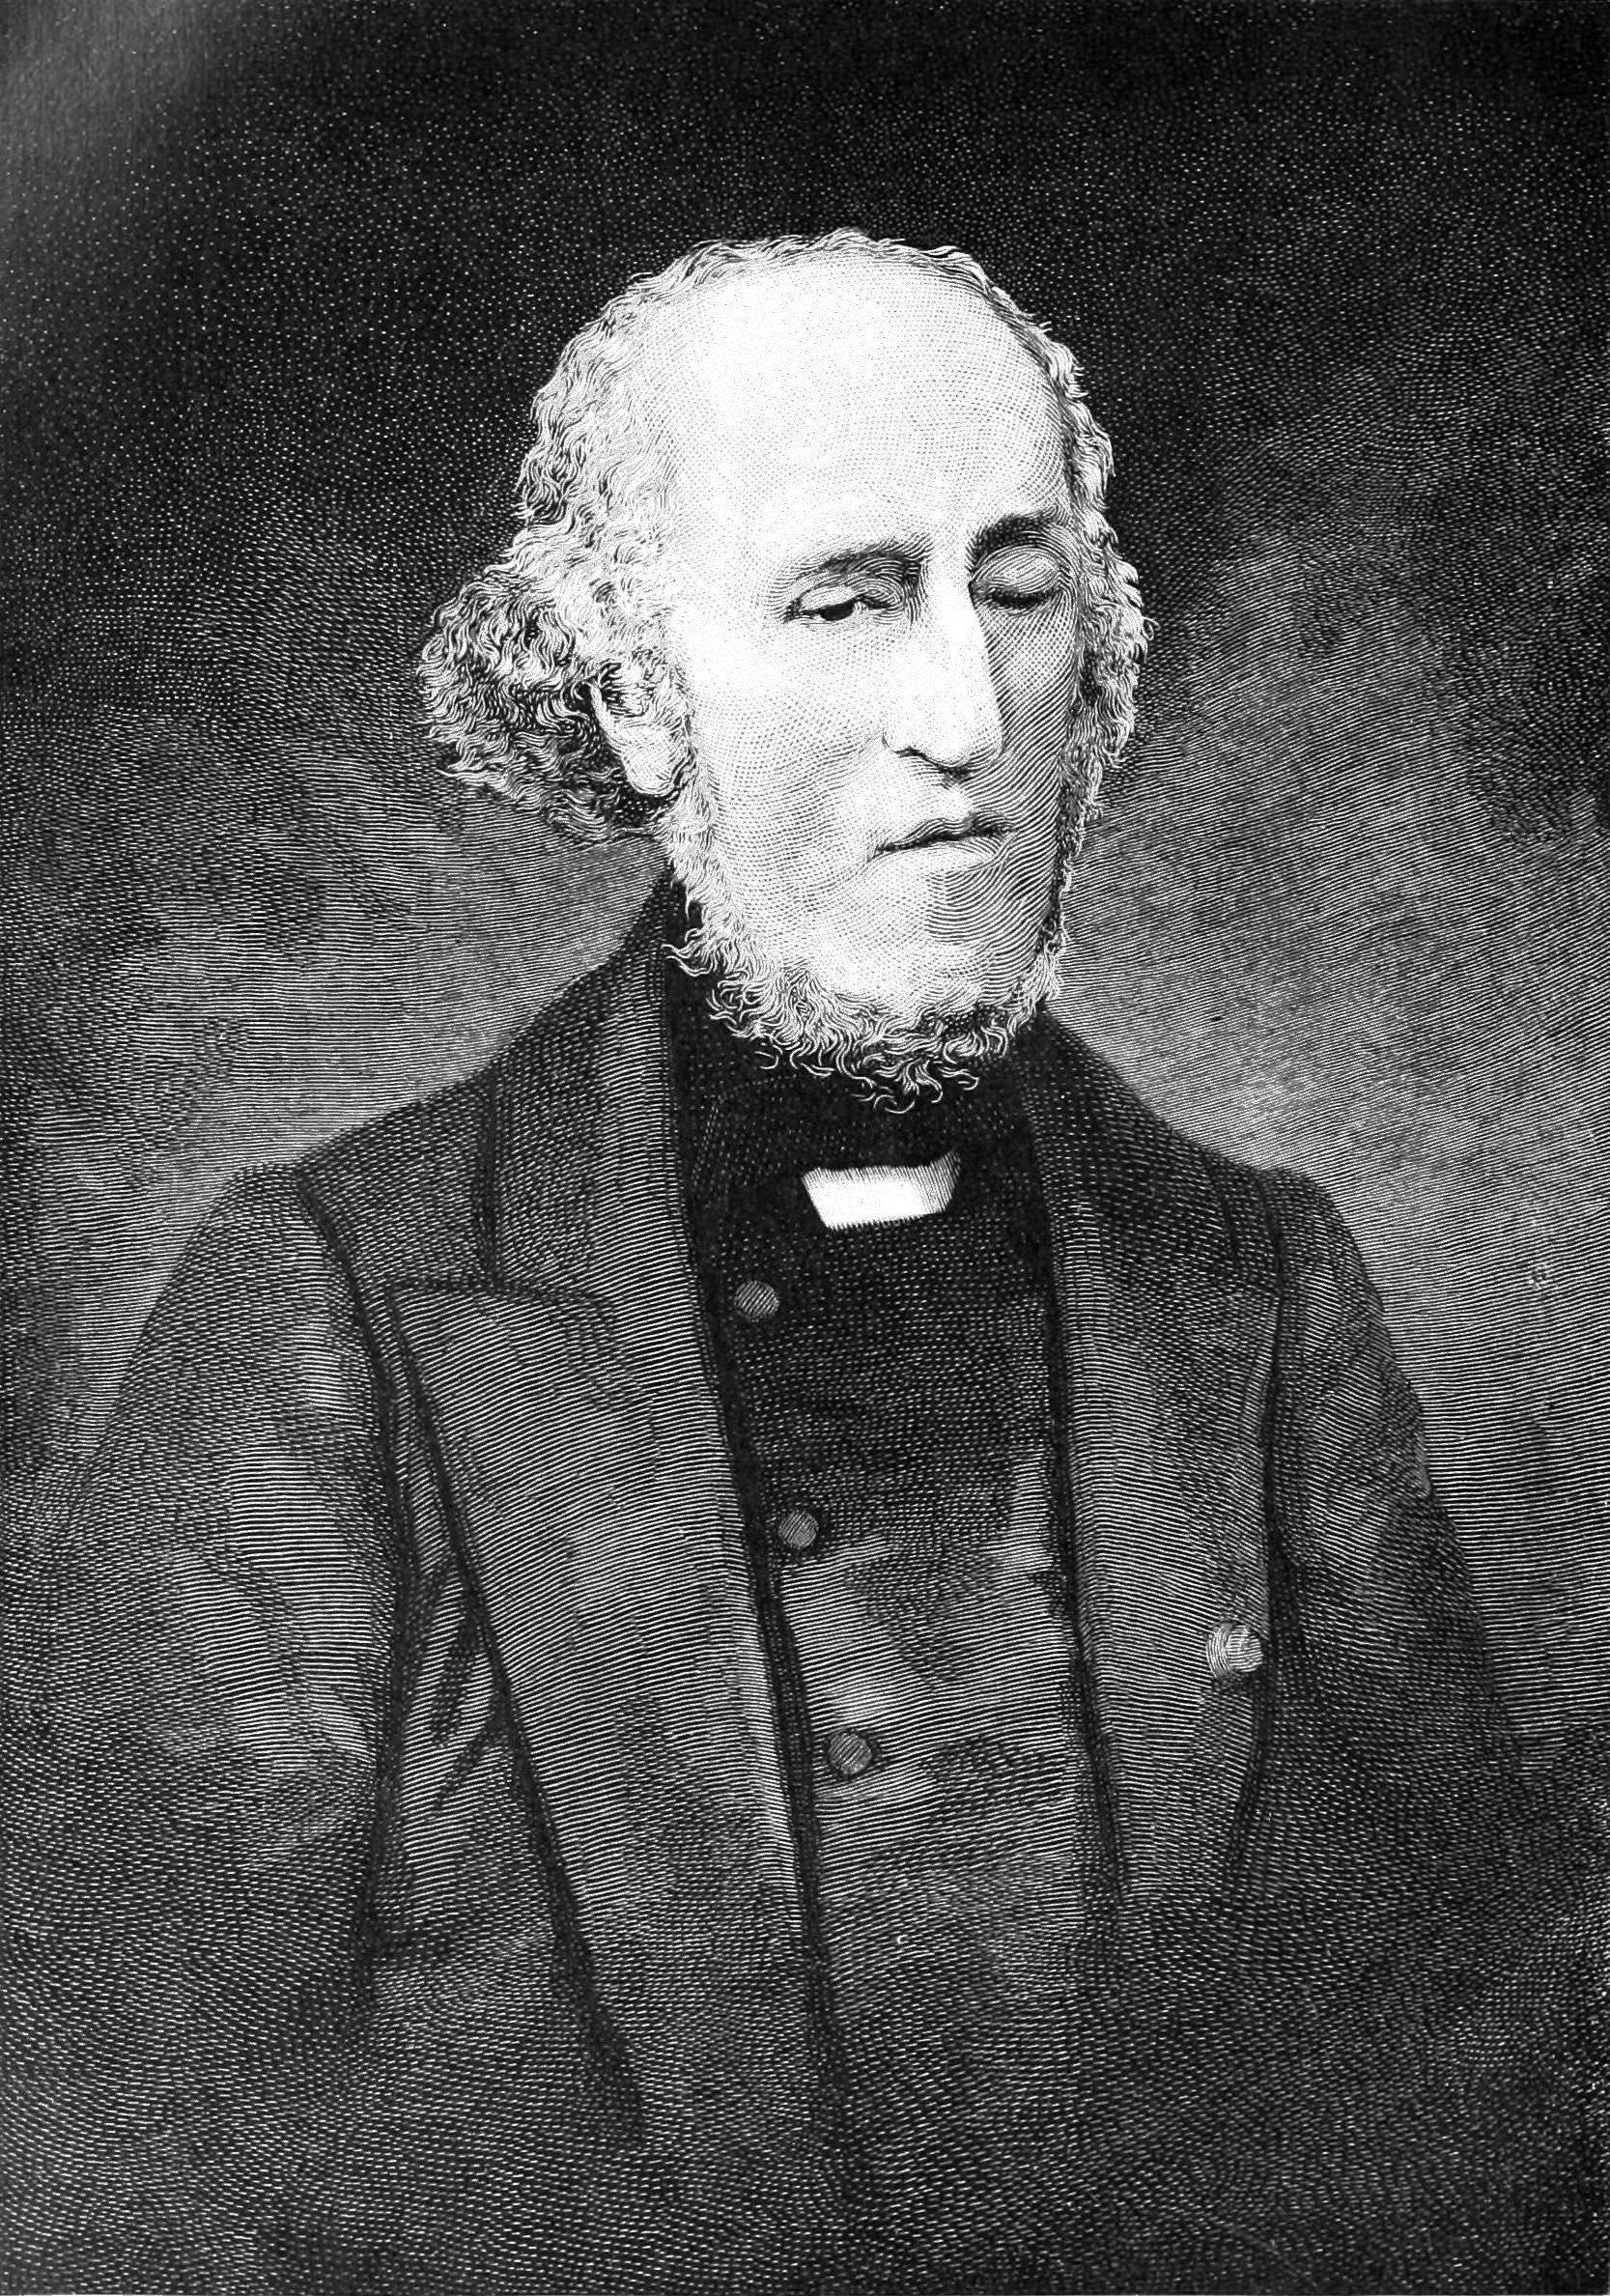
\includegraphics[height=300px]{img/Плато.png}}
	\caption{Слева -- \textit{Патрик Д'Арси}, Справа -- \textit{Джозеф Плато}}
\end{figure}

Анортоскоп представлял собой диск с анаморфным изображением,
которое можно было рассматривать как четкое неподвижное
изображение, когда диск вращался и просматривался через четыре
радиальные щели встречно вращающегося диска. Диски также могли
быть полупрозрачными и освещаться сзади через щели вращающегося
против часовой стрелки диска.

Далее был создан зоотроп, который оказался хорошей заменой
диску, описанному выше. «В зоотропе диск с отверстиями заменен
деревянным или металлическим барабаном, открытым сверху,
прорезанным вертикальными щелями по бокам и вращающимся
горизонтально на оси. Диск с картинками заменен длинной лентой,
которая помещается, свернутая в круг, внутри барабана. Эти ленты
могли вместить пять, десять и более дюжин картинок, тогда как диски
не могли вместить больше двух дюжин.» — Жорж Садуль. Вот мы и
подобрались от истории создания эффекта до использования этого
эффекта в реальной жизни.

\newpage

\section{Природные условия, объясняемые персистенцией}

\subsection{Молния}

При грозе люди обычно видят молнии как большой электрический
разряд из неба. На деле мы чаще всего видим траекторию движения –
остаточное изображение из-за очень яркого белого света.

\image{Гроза.jpg}{230}{След молнии на фоне темного неба}

\subsection{Снежные бури}
В снежную метель иногда становиться сложно увидеть, что
находиться даже в метре от вас. Это возникает не только от того что
одновременно падает огромное количество снежинок, но и от того, что
снежинки преломляют свет, и мы видим свет уже упавших снежинок,
как свет ещё падающих.

\image{Снег.png}{230}{Снежная метель}

\newpage

\section{Прямые использования эффекта}
\subsection{Тауматроп}

Таумотроп - это игрушка, основанная на оптической иллюзии: при
быстром вращении кружка с двумя рисунками, нанесенными с разных сторон,
они воспринимаются как один. Была особо популярна в Викторианскую эпоху.
Жорж Садуль утверждает, что создателем тауматропа является Джон
Гершелл. Ещё в 1824 году он поспорил со своим другом Чарльзом Беббиджем,
что сможет показать ему одновременно две стороны золотой гинеи. Он
вращал монету на ребре, а Беббиджа попросил поместить глаз на её уровне.
Обе стороны монеты слились воедино.

В 1825 Генри Фиттон и доктор Пари, популяризируя этот опыт, превратили
его в детскую игрушку, получившую имя тауматроп.

\image{Пингвин.jpg}{182}{Таумотроп с пингвином в шаре}

\subsection{Анортоскоп}

Анортоскоп — аппарат изобретённый в 1828 году брюссельским
физиком Жозефом Плато.

Анортоскоп состоял из двух дисков: прозрачного, помещённого сзади, и
непрозрачного помещённого впереди и имевшего отверстия. Оси дисков,
находились рядом, но не совпадали и которые приводились во вращение
вокруг одной и той же оси, во взаимно противоположном друг другу
направлении и с различными скоростями. Передний непрозрачный круг
снабжен вырезами, на заднем же, прозрачном и освещаемом помещенной
позади его свечкой, находится рисунок, который, будучи наблюдаем сквозь
щели переднего круга во время вращения кругов, появляется при известном
отношении скоростей вращения обоих кругов.

Анортоскоп создавал впечатление, как говорил Плато: «точного изображения
гиперболы, проходящей через два центра вращения». Позже он заменял одну
из линий рисунками, таким образом получая искаженное изображение вместо
правильной линии.

\image{С мышкой.jpg}{150}{Анортскоп, вышитый 13-летним мальчиком для школьного проекта}

\newpage
\thispagestyle{fancy}
\renewcommand{\sectionmark}[1]{\markright{#1}}
\fancyhf{}
\fancyhead[R]{\bfseries\thepage}
\fancyhead[LO]{\bfseries Прямые использования эффекта}
\subsection{Фенакистископ и стробоскоп}
Фенакистископ — лабораторный прибор, конструкция которого
основана на персистенции, способности сетчатки человеческого глаза
сохранять изображения. Изобретателем фенакистископа является Жозеф
Плато. Почти одновременно с Плато Симон фон Штампфер изобрел аппарат,
очень похожий на фенакистископ и назвал его «стробоскопом». Является
более совершенным анортоскопом.

\image{Фенакистископ.jpg}{172}{Обычный фенакистископ}

\subsection{Зоотроп}
Я уже упоминал зоотроп в истории создания персистенции, так что
пришло время рассмотреть это подробнее.

Зоотроп — устройство, конструкция которого основана на персистенции,
способности сетчатки человеческого глаза сохранять изображения.


Изобретателем зоотропа является Уильям Джордж Хорнер. Зоотроп является
трансформацией фенакистископа Жозефа Плато.


Современный зоотроп был изобретен в 1833 году британским математиком
Уильямом Джорджем Хорнером. Сам он назвал свое изобретение «дедалеум»
или «колесо дьявола». В 1860 году француз Дезвинь, и американец Уильяма Е.
Линкольн закрепили за всеми подобными устройствами название «зоотропа».


В 2008 году компания Sony создала зоотроп в виде тора диаметром 10 метров
и 10 тонн весом. Внутри находится второй тор, представляющий собой
большое количество выгнутых экранов. Внутренний тор вращается с
окружной скоростью 44 км/ч (и может разгоняться свыше 50 км/ч). На экранах
же появляется высокочёткое изображение.


Зоотроп был занесён в книгу рекордов Гиннесса, как самый крупный в мире.
(Посмотреть на него можно будет в презентации)

\image{зоотроп.jpg}{172}{Чертеж одного из первых зоотропов в мире}

\newpage

\subsection{Кинеограф}

Кинеограф— приспособление для создания анимированного
изображения, состоящего из отдельных кадров, нанесённых на листы бумаги,
сшитые в тетрадь. Зритель, перелистывая особым способом тетрадь,
наблюдает эффект анимации. Кинеография является одной из форм
мультипликации.


Название кинеограф запатентовано в 1868 году англичанином по имени Джон
Бернс Линнет. В 1894 году пионер кинематографа Макс Складановски
использует кинеограф для просмотра своих первых пробных съёмок.


В 1897 году англичанин Генри Уильям Шорт наладил массовое производство
кинеографа под патентованным названием филиоскоп, снабдив его
металлическим футляром и рычагом, облегчающим перелистывание страниц.

\image{Кинеограф.jpg}{300}{Нарисованный кинеограф}

\subsection{GIF}

GIF — растровый формат графических изображений. Способен хранить
сжатые данные без потери качества в формате не более 256 цветов. Не
зависящий от аппаратного обеспечения формат GIF был разработан в 1987
году (GIF87a) в фирме CompuServe для передачи растровых изображений по
сетям. В 1989-м формат был модифицирован (GIF89a): были добавлены
поддержка прозрачности и анимации). Долгое время GIF был одним из
наиболее распространённых форматов в интернете. GIF позволяет соединять
и демонстрировать в виде видео отдельные фотографии.
\newpage
\section{Косвенные использования эффекта}
\pagestyle{fancy}
\renewcommand{\sectionmark}[1]{\markright{#1}}
\fancyhf{}
\fancyhead[R]{\bfseries\thepage}
\fancyhead[LO]{\bfseries\rightmark}

\subsection{Кадровая частота}

Кадровая частота используется в абсолютно всех экранах и мониторах,
это специальная величина которая измеряет сколько кадров монитор покажет
в секунду. Когда монитор показывает много кадров мы видим целое, не
склеенное видео. Тут инерция зрения возникает как косвенный эффект. Как
интересный факт стоит отметить то что до 1922 года инерция зрения
считалась основным эффектом зрения, который используют в фильмах, но
затем было доказано обратное.

\image{Медведь.jpg}{100}{Один шаг анимированного медведя (покадрово)}

Нестандартные (дополнительные) примеры: Электронные часы, электронные
билборды, видео.

\subsection{POV пропеллер}

И вот мы подобрались к самому интересному: POV механизмы. Каждый
из нас замечал на детских праздниках светящиеся пропеллеры. Они состоят
из простого мотора и нескольких светодиодов. Дело в том, что если
посмотреть на этот пропеллер со стороны науки, то он опережает свое время.
Он не только дает красивый зрительный эффект, но и преображает
одномерную полоску светодиодов в двумерный рисунок. Впоследствии
именно это стало отправной точкой моего продукта.

\image{пропеллер.jpg}{300}{POV пропеллер}

\newpage

\section{Практическая часть}
\subsection{Введение в практическую часть}

Любой проект начинается с идеи. Мой проект тоже начался с идеи.
Точнее с одной идеи и огромного количества предположений по возможной реализации продукта.
Что-бы как-то объединить все соображения в один продукт я набросал список, того,
что понадобится для физической реализации голограммы:
\begin{enumerate}
	\item Кривошипно-шатунный механизм
	\item Мотор
	\item Светодиоды
	\item Управление системой
\end{enumerate}
\subsubsection{Кривошипно-шатунный механизм}

Кривошипно-шатунный механизм(КШМ) предназначен для преобразования
возвратно-поступательного движения поршня во вращательное движение
(например, во вращательное движение коленчатого вала в двигателях
внутреннего сгорания), и наоборот. Детали КШМ делят на две
группы, это подвижные и неподвижные детали:

Подвижные: поршень с поршневыми кольцами, поршневой палец,
шатун, коленчатый вал с подшипниками или кривошип, маховик.

Неподвижные: блок цилиндров (является базовой деталью двигателя
внутреннего сгорания) и представляет собой общую отливку с картером,
головка цилиндров, картер маховика и сцепления, нижний картер (поддон),
гильзы цилиндров, крышки блока, крепежные детали, прокладки крышек
блока, кронштейны, полукольца коленчатого вала.

Конечно это общее определение и устройства КШМ. Мне КШМ нужен для того,
чтобы привести платформу со светодиодами в движение.

\image{Шатун.png}{350}{Устройство КШМ}

\newpage

На Рис.13 изображена примерная модель моего шатунного механизма
Как видно он состоит из 4 деталей:
\begin{enumerate}
	\item Крепление 1 шатуна к мотору
	\item 1 шатун
	\item 2 шатун
	\item Крепление 2 шатуна к платформе
\end{enumerate}
Точками BMT и НМТ обозначены самое высокое
положение платформы и самое низкое соответственно.
Между ними расстояние S к которое я вычислю позже.
Шатунный механизм получилось сделать достаточно просто
из маленького кусочка орг-стекла и пару отрезков проволоки.

\subsubsection{Мотор}

Понятно, что шатунный механизм надо привести в движение
при помощи мотора.
Сначала я подумал реализовать мотор без каких-либо затрат,
с помощью дрели и крепежей, но затем я нашел неплохой вариант
мотора из СССР.

\image{Мотор.jpg}{160}{Мотор}

Крутящиеся части у него с 2 сторон, поэтому можно сделать целых 2 шатунных механизма
с одной и другой стороны. Питание может происходить от розетки без адаптеров питания.
В начале проекта это было довольно удобным дополнением, но затем пришлось помучаться
(см. 8.4.3).

\subsubsection{Светодиоды}

Светодиоды -- самая главная часть моего продукта
изначально идея заключалась в том, чтобы сделать маленькую
матрицу из RGB\footnote{\ RGB -- red green blue(красный зеленый синий)} светодиодов.

\image{Светодиод.png}{140}{RGB светодиод}

\newpage
На картинке видно, что у каждого светодиода есть 4 ножки. Если на первую подать
плюс а на вторую минус, то загорится красный цвет. Если на третью подать
плюс а на вторую минус, то загорится зеленый цвет. Если на четвертую подать
плюс а на вторую минус, то загорится синий цвет.

\begin{figure}[ht]
	\center{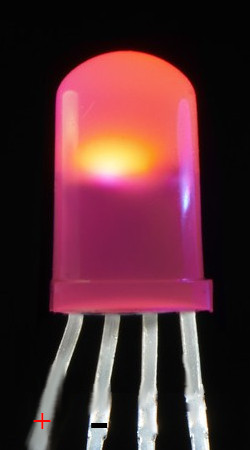
\includegraphics[height=160px]{img/Светодиод красный.jpg} }
	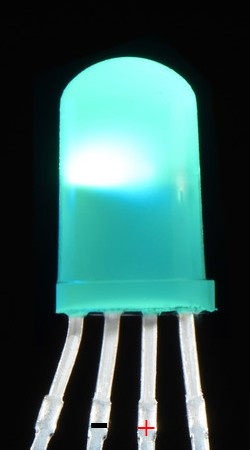
\includegraphics[height=160px]{img/Светодиод зеленый.jpg}
	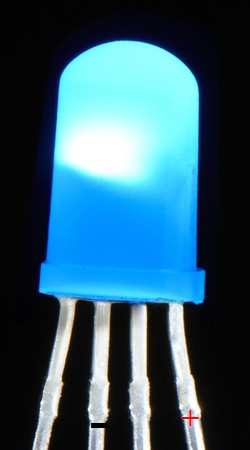
\includegraphics[height=160px]{img/Светодиод синий.jpg}
	\caption{\textit{RGB светодиод, горящий красным, зеленым и синим цветом}}
\end{figure}

И так теперь у нас есть 3 цвета: красный, зеленый, синий.
Теперь смешаем цвета: из красного и синего получим фиолетовый,
из красного и зеленого -- желтый, из зеленого и синего -- голубой.
Если соединим все три ножки, то получим белый.
И так у нас есть практически вся палитра радуги(за исключением оранжевого)
и белый цвет. При всех этих обстоятельствах я подавал ток с фиксированным напряжением
3V. Но производители заявляют, что на RGB светодиоды можно подать от 2,1V до 3,3V но
как можно было догадаться если мы будем подавать ток с меньшим напряжением, то светодиоды
будут гореть тускло, а с большим ярко. В аналоговых входах моего МК
\footnote{\ МК -- микроконтроллер(подробнее в 8.1.4)}
напряжение можно подавать деля его на десятые. Таким образом получаем, что у 
нас есть есть 23 напряжения и 7 цветов для каждого напряжения. Вычислим 
количество цветов и оттенков К, которые мы можем получить $$K=23!\times 
7\thickapprox 1,8*10^{23}$$ Конечно мы не увидим каждый из оттенков и они нам 
попросту не нужны в настолько большом сегменте. Возьмем общепринятое количество 
оттенков каждого цвета -- 256. Тогда для того, что-бы запрограммировать 1 
светодиод нам понадобится передать коду L значений. Вычислим L: $$L=256\times 
256\times 256= 16777216 \thickapprox 1,6*10^7$$ Ученые-биологи пока доказали, 
что человек может воспринимать около 10 миллионов ($10^7$) цветов, поэтому для 
школьного проекта такой палитры цветов будет более чем достаточно.

Это все начальные данные о светодиодах, которые необходимо знать не только для 
того,чтобы понять, но и для того, чтобы повторить проект.

\subsubsection{Микроконтроллер}

Из текста о светодиодах можно было понять, что для управления ими нужен 
источник питания источником питания может служить простой адаптер для зарядки 
гаджетов, но тогда, что-бы включить или выключить светодиод нам придется 
совершать определенные механические действия. Но человечество давно изобрело 
процессоры, которые помогают из несложного набора единиц и нулей начать или 
прекратить подачу энергии на определенные участки пути. Конечно, использовать 
голый процессор в моем проекте было бы сложно и не очень нужно: ведь процессору 
нужна и память, и программатор, и ядро, написание которого может занять годы.

Поэтому предлагаю вашему вниманию список, состоящий из названий микросхем в 
корпусе которых это объединено:

\begin{enumerate}
	\item   Микрокомпьютер
	\item   Компьютер
	\item   Микроконтроллер (МК)
\end{enumerate}


\newpage
Давайте поподробнее разберем все 3 варианта и в конце, сопоставив все, выберем 
самый лучший. Для этого я составил таблицу, которая показывает 3 главных 
аспекта: кол-во портов, память и удобство программировать.
\begin{center}
\begin{small}
\begin{tabular}{ |c|c|c|c|c|}
	\hline
	Название        & Определение            & Кол-во портов    & Память      & Программирование        \\ \hline

	Микрокомпьютер  & Семейство компьютеров, & 12-46            & 8-256 ГБ    & удобные среды           \\
	                & которые в отличии      &                  &             & разработки              \\
	                & от других компьютеров  &                  &             & непосредственно         \\
	                & работают на            &                  &             & в микрокомпьютере       \\
	                & RAM-архетиктуры.       &                  &             &                         \\ \hline

	Компьютер       & Здесь: система,        & 2-8 портов USB-A & 256-2048 ГБ & Практически нету        \\
	                & имеющая полноценный    &                  &             & открытых средств        \\
	                & процессор, способный   &                  &             & разработки, все команды \\
	                & выполнять миллиарды    &                  &             & по управлению USB       \\
	                & операций в секунду     &                  &             & можно осуществить       \\
	                &                        &                  &             & только через терминал   \\\hline

	Микроконтроллер & Микрокомпьютер         & 12-56            & до 1ГБ      & среда разработки        \\
	                & с урезанным            &                  &             & Arduino idle            \\
	                & функцианалом           &                  &             &                         \\
	\hline
\end{tabular}
\end{small}
\end{center}
Давайте разберемся по порядку: я беру микроконтроллер для удобства его
программирования также у него должно быть достаточное кол-во портов для
подключения всей электроники, о которой речь пойдет позже, так что компьютер,
не смотря на его большую вычислительную мощность не подходит.

Так же мне ни к чему покупать микрокомпьютер т.к. с таким проектом может 
справится сравнительно небольшой микроконтроллер. На нем я и остановился, а 
именно на модели Arduino NANO.

\image{дуня нано2.jpg}{140}{Arduino NANO}

Пусть на такой микроконтроллер провода нужно будет припаивать, но по моему 
опыту это один из самых удобных МК из всех. Так же следует отметить, что 
Arduino NANO - уменьшаная копия Arduino UNO, так что в последствии я буду 
использовать обе модели для наглядности, разницы между ними нет. На Рис. 17 
представлена распиновка (последовательность входов и выходов МК). Стоит 
отметить, что даже на таком маленьком микроконтроллере я не использую все 
выходы, а лишь несколько цифровых (помеченных надписью Dig).

\image{дуня нано.jpg}{150}{Распиновка Arduino NANO}

\subsubsection{Светодиодная матрица}

А теперь перейдем к решению вопроса, который я старательно обходил в 8.1.3:
если у светодиода 4 ножки, то ему понадобится 4 пина?

Да это так, а т.к. мой продукт должен состоять не из одного светодиода, а
как минимум 4, то их ножки займут все 12 цифровых выходов(+) и 1 землю(-).
Но голограмма 4$\times$4$\times$4 будет слишком маленькой. В идеале размеры
голограммы должны составлять 16$\times$16$\times$16. Но тогда ножек у
светодиодов будет $16*16*3=768$, что в 64 раза больше, чем есть у меня на 
плате, и в 15 раз больше, чем на самом большом МК, который подается сегодня.

Рассмотри RGB ленту:Начнем с того, что в обычной светодиодной ленте, все светодиоды ленты
питаются и светятся одновременно, поскольку все они получают питание
параллельно от одного источника, драйвера, который работает по своему алгоритму, реализуемому
непосредственно внутри драйвера, и просто подает питание сразу на всю ленту, по сути - на все
параллельно подключенные к нему светодиоды.

Адресная светодиодная лента, в отличие от обычной, содержит так называемые адресные
светодиоды. Это значит, что каждый светодиод хотя и получает питание параллельно от
общего источника, включается каждый светодиод по индивидуальной команде, и значит,
на каждом светодиоде можно получить собственный уникальный оттенок, один из 16581375
возможных(см.8.1.3).

Каждый светодиод в адресной ленте имеет свой уникальный адрес, по которому
драйвер обращается к нему при помощи трехбитной команды. Команды отправляются в
линию последовательно, для этого служит третий на ленте провод «DATA INPUT».

\image{лента.jpg}{80}{Распиновка адресной ленты}=

Возле каждого светодиода на адресной ленте установлен свой микрочип.
Каждый чип имеет три выхода — каждый на свой цвет, вход передачи данных,
выход передачи данных, вывод питания, вход установки режима и общий вывод.

Каждый RGB-светодиод на самом деле имеет в себе три светодиода (красный,
зеленый и синий), поэтому для управления одним сегментом (один сегмент — это
RGB-светодиод с чипом) требуется 3 байта информации, один байт — один цвет.

Каждый байт может принимать одно из 255 значений, поэтому в принципе каждый
RGB-светодиод способен дать свет одним из 16581375 оттенков. Количество байт
в одной команде равно таким образом 3 умножить на количество последовательных
рабочих сегментов в ленте. Конечно можно передавать ленте каждый раз по 3
значения, но я думаю, что удобнее всего будет передать ей один цвет в формате
hex(16-битный формат представления цвета, где каждый цвет кодируется 2 
символами).

%Но как можно было понять что-бы сделать из ленты матрицу надо разрубить 256
%светодиодную ленту на 16 кусочков по 16 светодиодов, а затем соединить их
%последовательно.

\image{лента в тинкеркад.png}{180}{Макет адресной марицы, созданный мной}

\newpage

\subsection{Корпус}
И так мы определили все, что нужно для реализации продукта.
теперь надо подумать как это все компактно уместить под крышку
одного корпуса.
\subsubsection{Размеры}
Конечно сначала нужно поговорить о размерах корпуса,ведь принцип
чем больше - тем лучше я думаю не подходит. И так структурируем каждую
деталь корпуса. Стоит отметить, что под корпусом я подразумеваю только
неподвижные детали, о шатунном механизме, моторе и других деталях я
напишу позже.

Хочется отметить, что на этот момент у меня уже есть все вещи, которые описаны
в 8.1, поэтому я могу совершенно спокойно снять все замеры именно с них.
%!таблица размеров
Внимательно изучив таблицу я понял, что платформа, на которую будет крепится
сама модель должна быть размером 16$\times$22, что-бы на ней поместилась
матрица и дополнительные крепления. К слову матрицу я сделал не сам, как
первоначально задумывал, а купил в китае, т.к. цена на ленту с таким же
количеством светодиодов была даже выше, чем цена на матрицу(подробнее 8.8.3)

Далее изучив размер мотора, я понял, что коробка корпуса должна быть высотой в
20см. Таким образом я набросал примерный план некоторых деталей для статической
части корпуса.
\\
\begin{center}
	\begin{tabular}{ |c|c|c|c|c|}
		\hline
		Номер  & Количество & Материал & Размеры(мм)             \\
		детали & деталей    &          &                         \\
		\hline
		1      & 2          & фанера   & 220$\times$200$\times$5 \\
		\hline
		2      & 3          & фанера   & 160$\times$200$\times$5 \\
		\hline
		3      & 4          & брус     & 20$\times$200$\times$10 \\
		\hline
		4      & 4          & стальной & 320$\times$8            \\
		       &            & стержень &                         \\
		\hline
	\end{tabular}
\end{center}
\ \\
Предлагаю разобраться в этой таблице подробнее.\\
\subsubsection{Детали 1-2}

Первые две детали будут образовывать коробку, в которой будет находится
электроника и шатунный механизм. Вы, наверное, заметили, что вторых деталей
я сделал в количестве трех штук. Я сделал их именно столько для использования
внутренней перегородки о которой я рассажу позже. Изначально я хотел сделать
эти детали из гипсокартона.

\image{гибсокартон.jpg}{230}{Фото гибсокартона, который я использовал}

Этот материал оказался довольно плохим и не практичным к использованию,так что
сделать из него что-либо у меня не получилось.

%!детали из гибсокартона

Далее я нашел относительно хороший лист фанеры и наметил все 5 деталей.

\image{разметка фанеры.jpg}{180}{Разметка фанеры}

Потом начался процесс выпилки. Пилить такое дерево можно практически абсолютно
всем начиная от фрезы заканчивая ручной пилой.Я выбрал относительно легкий
вариант -- электролобзик. Им достаточно легко пилить и получается относительно
маленькая погрешность: всего 0,3мм. Выпилил я все за один зимний вечер и
получилось все с первого раза.

\image{разметка фанеры.jpg}{180}{Выпиленные детали}

Дальше начался процесс сборки.Он состоял в том, что надо было разметить  Он был
относительно сложным, т.к фанера имела маленькую ширину.

%!два уголка,которые у меня получились в первый раз

При вворачивании очередного самореза фанера сломалась. Тогда
я понял, что нужно все переделывать и делать дополнительные подпорки для
каждого угла фанеры.

\subsubsection{Дополнительные подпорки (3-я деталь)}

Для изготовления подпорок я выбрал брус, длиной 2 метра, который я распилил
на 4 кусочка по 20см каждый. Вот что получилось у меня в итоге:

%! распиленный брус

Конечно можно было мучиться с уголками, но брус выполнял еще одну немаловажную
роль для продукта -- в нем можно было установить держатели для подложки.

\subsubsection{Держатель подложки (4-я деталь)}

Чем я и занялся. Дело в том, что прутья, которые я хотел купить не продают
настолько маленьких размеров, так что за идеально ровными прутьями мне пришлось
ехать на другой конец города -- на металлолом.

%!прутья из металлолома

Но как можно видеть на фото из этого вытекает целых 2 проблемы: первая, что
прут покрыт ржавчиной, вторая, что он один и большой -- значит прийдется
пилить.

С первой проблемой справился довольно быстро: воду и перекись смешиваем в
пропорции $\frac{2}{1}$ и добавляем лимонную кислоту 100 грамм на 200 мл
перекиси. Оставляем так на час и ржавчины нет.

%!ржавчина уходит

Со второй проблемой пришлось помучаться: сталь плохо пилится ручной пилой,
а пилы по железу для лобзика у меня нету. В начале я распилил прут на 4 части
по 32 см, но затем оказалось, что это слишком много и прут пришлось подпиливать
после установки.

\subsubsection{Сборка}

Сборка прошла на удивление гладко, в два этапа.

В первый этап я просверлил отверстие в детали 3 диаметром 8 мм, затем
начал забивать деталь 4 в деталь три.

%!одна деталь 4 в детали 3

Далее я повторил свю эту операцию еще три раза. Самое сложное было просверлить
отверстие идеально ровно под углом $90^/circ$.

%!4 детали

Осталось прикрутить все вместе. Вот полученный результат:

%!результат

\subsubsection{Покраска}
\newpage

\subsection{Динамические детали корпуса}


\subsection{Дополнительные технические улучшения}

\subsubsection{Щелевой оптический датчик}

Конечно многие могли заметить то, что я избегаю сложных вычислительных
задач в этом проекте и не очень хочу заниматься некоторыми расчетами. Это все
верно, но с помощью оптического датчика можно решить достаточно много проблем
которые могут возникнуть при работе с проектом. Во-первых неравномерность
шатунного механизма. Нетрудно догадаться, что под силой притяжения шатун будет
быстрее спускаться, чем подниматься. Во-вторых могут возникнуть проблемы
в прорисовке и картинка будет сбиваться. В-третьих вычислительная мощность МК
маленькая и все ОЗУ во время прорисовки будет заполнено, так что решать
проблему путем физических вычислений по любому не получится. Тут на помощь
приходит датчик движения. Но не простой. Дело в том, что скорость передачи
датчиков очень мала. Она мала настолько, что просто не возможно что-либо
передать МК на больших скоростях, которые я планирую развить. Поэтому я буду
использовать щелевой датчик движения(щелевой оптический датчик) из названия
которого можно понять, что радиус его поля всего лишь щель.

В данный датчик состоит из лазера и фотоэлектрического датчика: лазер постоянно
светит через через щель, а фотоэлектрический датчик принимает его свет и
выдает нули, если фотоэлектрический датчик перестает принимать свет т.е. между
ним и лазером возникает препятствие, то датчик передает единицы. В нашем случае
препятствие -- нижнее положение шатуна. Таким незамысловатым образом я могу
где находится шатун в определенный промежуток времени.

%!фото датчика

\subsubsection{Светодиоды}

Для понимания состояния МК я решил добавить на корпус зеленый и желтый 
светодиод.\\
\textbf{$\text{Зеленый}$}

Зеленый светодиод я планирую использовать в 2 режимах: первый когда он 
горит это означает, что плата работает, прорисовка запущена. Второй когда он 
мигает это означает, что плата готовится к запуску. Стоит отметить, что если
светодиод мигает слишком долго -- это означает, что плата не смогла произвести
калибровку и/или возникла ошибка при запуске мотора(см.8.4.3).

%!зеленый светодиод
\textbf{$\text{Желтый}$}

Желтый светодиод будет гореть при всех остальных проблемах и мигать, если будет
загрузка на плату.

%!желтый светодиод

\subsubsection{Реле для мотора}

Реле в моем проекте играет довольно большую роль. Как я говорил в 8.1.2
чтобы связать мотор и МК так, что МК будет управлять мотором нужно реле.

%!фото реле

Реле -- автоматический переключатель, который может переключить даже маленькая
сила тока. Предлагаю разобраться в его устройстве подробнее:

%!устройство реле

Реле представляет собой катушку, состоящую из немагнитного основания, на 
которое намотан провод из меди с тканевой или синтетической изоляцией, но чаще
всего с диэлектрическим лаковым покрытием. Внутри катушки установленной на 
нетокопроводящее основание, размещается металлический сердечник. Также в 
устройстве имеются пружины, якорь, соединительные элементы и пары контактов.
 
При подаче тока на обмотку электромагнита (соленоида) сердечник притягивает 
якорь, который соединяется с контактом и электрическая или электронная цепь 
замыкается. При снижении силы тока до определенного значения, якорь, под 
действием пружины, возвращается на исходную позицию, вследствие чего 
происходит размыкание цепи.

Более плавная и точная работа достигается благодаря использованию резисторов,
а защиту от скачков напряжения и искрения обеспечивает установка конденсаторов.
У большинства электромагнитных реле имеется не одна, а несколько пар 
контактов, что позволяет управлять несколькими цепями одновременно.

Далее мы будем говорить о самом важном аспекте моего продукта -- 
программировании. Но перед тем, как я приступлю рассказывать, я хочу отметить,
что в этой и последующих главах встречается программный код. Оформил я его так:
слева идет код, а справа комментарии и пояснения.

Первым делом я решил запрограммировать матрицу.\newpage
\subsection{Программирование матрицы}
Первый код дался мне довольно легко: всего неделя изучений и улучшений. Предлагаю
вашему вниманию первый рабочий код для светодиодной матрицы.
\begin{flushright}\begin{huge}\textcolor{grey}{Arduino}\end{huge}\end{flushright}
\begin{tabular}{c p{180px}}
\hline
\begin{lstlisting}[style=myLatexStyle]
#include "Adafruit_NeoPixel.h"
const uint32_t AR[16][256] PROGMEM = 
#define PIN 13        
#define NUM_LEDS 256   
Adafruit_NeoPixel strip = Adafruit_NeoPixel(
    NUM_LEDS, PIN, NEO_GRB + NEO_KHZ800);
void setup() {
    strip.begin();
    strip.setBrightness(50);    
    strip.clear();                          
    strip.show();                           
	}
void loop() {
    for (int i1 = 0; i1 < 16; i1++){
			for (int i = 0; i < 256; i++){
				strip.setPixelColor(i,
					pgm_read_word(&AR[i1][i]));
				};
			strip.show();
			delay(100);
		};
	}
\end{lstlisting}
&
\begin{tabular}{p{180px}}
Импортируем библиотеку\\
Задаем массив данных\\
Описываем переменную порта\\
Описываем переменную для свет.\\
Описываем переменную библиотеки
на которой управляется матрица\\
Начинаем ф-цию установки\\
Начинаем общение с матрицей\\
Устанавливаем яркость(0-255)\\
Очищаем матрицу(заливаем черным)\\
Показываем результат заливки\\
Заканчиваем установку\\
Начинаем постоянную ф-цию\\
Берем цикл для слоев\\
Берем цикл для светодиодов\\
Устанавливаем значение 
текущего светодиода\\
Заканчиваем цикл светодиодов\\
Показываем слой\\
Ждем 100мс\\
Заканчиваем цикл слоев\\
Повторяем постоянную ф-цию \\
\end{tabular}\\
\end{tabular}

\subsubsection{Почему  Adafruit NeoPixel(ст. \#1)}

Для начала предлагаю разобрать все возможные варианты управления матрицами:
через библиотеки и на прямую. Я думаю, что и вам и мне выбор сразу очевиден --
пойти не через библиотеки, т.к. они занимают много ОЗУ и мало для чего будут
нужны. Но тут не все так просто. Пойдя вторым способом я наткнулся на огромное
количество подвисаний с которыми не собирался сталкиваться.

Вывод очевиден: оказывается библеотеки ко всему прочему оптимизируют программу 
не давая ей повода зависать. Тут перед нами открывается еще один выбор: 
использовать fastLED -- вроде как более универсальную, но новую, не изученную
библиотеку или старую NeoPixel от компании Adafruit. Думаю по моей работе можно
смело заявить, что я не ищу легких путей, поэтому я принялся "грызть" 
документацию по fastLED. Но вот прошло некоторое время и наступили каникулы. 
Моя семья и я уехали отдыхать и доступа к Arduino у меня не было, но я не 
отчаялся и использовал приложение Tinkercad в котором не было матрицы и я её
сделал собственными руками. Результат работы можно посмотреть на Рис. 20.
И тут возникла еще одна проблема: в Tinkercad нету поддержки fastLED, зато
старушка NeoPixel подключается и работает спокойно. Вот так я, перепробовав
кучу вариантов, выбрал самый неочевидный для себя. Под конец программирования 
вся среда разработки выглядела так:

%!среда разработки
\newpage
\subsubsection{Работа с данными (ст. \#2)}

Если вы думали, что тут пойдет лучше -- нет. Оптимальным вариантом был бы 
трех мерный массив, но сложность последующего управления им бы зашкаливала,
так что я поставил перед собой задачу использовать одномерный, ну максимум 
двумерный массив.

Если вы не совсем понимаете о чем я, ничего сейчас всё объясню. Представим 1
пиксель в качестве куба:

%!куб

Тогда одна линия ленты -- 16 кубиков.

%!16 кубиков

Тогда вся матрица -- 16 линий по 16 кубиков.

%! лента

Но загрузка ленты идет так как она расположена т.е. последовательно, поэтому
можно всю матрицу объединить в ряд, состоящий из 256 кубиков. Каждый кубик
должен иметь свой цвет и даже не горящие светодиоды просто имеют цвет черный. 
Тогда можно создать массив цветов, состоящий из 256 значений. 
Конечно далее для оптимизации черные точки после перезаливки можно будет 
пропускать, но сейчас и так нормально.

Теперь же осталась лишь проблема слоев, которую надо было решать. Ну я пошел
по легкому пути и создал двумерный массив, т.е. массив слоев (16), в каждой
ячейке которого хранится массив цветов.

%!куб

Ну вот и всё подумал я, но все было не так гладко. Для понимания той темы, о
которой я хочу сейчас поговорить я предлагаю посмотреть на строчку из кода:
\begin{lstlisting}[style=myLatexStyle]
const uint32_t AR[16][256] PROGMEM = 
\end{lstlisting}

На деле это просто обрывок, сама она выглядит очень большой, так что вместить
сюда ее тяжеловато и, как я думаю, совсем не нужно. К тому же массив я вставлю,
но чуть позже. Разберемся сначала с левой частью. 

Для начала я должен сказать, что AR -- название массива.[16][256] -- описание 
всех ячеек. Теперь разберемся с типом. Как я уже упоминал цвет я буду вводить
в hex формате т.е в цифровом формате, но int -- слишком маленький тип для 
огромного количества цветов, поэтому предлагаю ознакомиться со всеми доступными
типами данных. Напоминаю, что цветов у нас должно быть 16777216.

\begin{center}
\begin{tabular}{|l|c|c|c|}
\hline
название&вес&диапазон&работа с\\
типа&(бит)&значений&терминалом\\
\hline
int&16 &-32768\dots32767&Serial\\
\hline
uint&16 &0\dots65535&Serial\\
\hline
int32\_t&32 &-2147483648\dots2147483647&Serial\\
\hline
uint32\_t&32 &0\dots4294967295&Serial\\
\hline
int64\_t&64 &$-2^{63}$\dots$2^{63}-1$&--\\
\hline
uint64\_t&64 &0\dots$2^{64}-1$&--\\
\hline
\end{tabular}
\end{center}
Как можно заметить int32\_t самый подходящий вариант,но поразмыслив понятно,что
цвет, который мы всегда будем задавать будет величиной положительной, так что
изходя из этого и что-бы легче находить проблем в коде я использовал uint32\_t.

И так, мы определили тип теперь немного теории о памяти: дело в том, что она у
нас ограничена и ОЗУ использовать для такой огромной переменной вообще нельзя.
У меня при загрузке возникла проблема переполнения памяти на 2000\%. Довольно 
много. Первая идея у меня, да и наверное у вас: купить дополнительный модуль 
памяти, но сейчас этот модуль довольно дорогой и ждать его из китая пришлось
бы долго. Так что будем обходиться средствами МК, немного полазив в интернете,
я понял, что у МК целых 4 памяти: ОЗУ, ПЗУ, PROGMEM, EEPROM. Ну с первыми двумя
все понятно одна оперативная, другая занятая скетчем и ядром. Остаются 2
обе они программируемые, отличие лишь в том, что PROGMEM это расширение для
ОЗУ, а EEPROM - ячеечная память, она имеет 255 ячеек, которые хранят 255 
значений, что не достаточно для нас (нужно 256, а это значит, что в одну 
ячейку прийдется убрать 16 цветов, что будет не очень удобно и определенно 
замедлит процесс прорисовки). Так как в первых версиях я планировал заменять 
рисунок путем перезагрузки данных в плату с компьютера, то я подумал, что 
сделать эту переменную еще и константой будет хорошей идеей, позже я откажусь
от этого.

\subsubsection{Переменная библеотеки (ст.\#3-6)}

Переменная библеотеки strip хранит данные о матрице и о том, что в нее надо
записать. Именно она является неким мостиком между программой и матрицей и 
поэтому она просто необходима именно в ОЗУ памяти. Так же я создал 
дополнительные переменные PIN и NUM\_LEDS , что-бы было легче ориентироваться в
коде. 

\subsubsection{Функция установки (ст.\#7-12)}

Думаю, что эти строчки и по комментариям ясны и  понятны, так что скажу только,
что эта функция выполняется лишь раз при загрузки в плату, далее она не 
выполняется.

\subsubsection{Постоянная функция (ст.\#13-22)}

Постоянная функция -- функция, которая, заканчивая свою работу обращается сама 
к себе и получается бесконечно рекурентный цикл. в начале этой функции мы 
задаем 2 цикла: цикл слоев и цикл света, затем в цикле света рисуем весь слой,
обращаясь к нашей переменной AR с помощью функции для чтения из PROGMEM памяти
pgm\_read\_word(). После окончания рисовки слоя просто выводим его и ждем пару
миллисекунд для прорисовки и рисуем следующий слой.

Вот и вся начальная функция, далее только её обновления и улучшения.

\subsubsection{lines.h или как связать МК и абсолютно любой ЯП}

Понятно,что такой огромный массив сложно читать не только МК, но и обычному
человеку. Поэтому я решил создать свою подбиблеотеку, в которой я как раз 
и опишу весь массив. Создание и подключение оказалось довольно легким, но это
не изменило одного факта: массив трудно читаем, а так как он трудно читаем, то
и управлять всей матрицей тоже не просто. Обобщим: нам нужна такая программа,
в которой можно будет не только легко читать массив, но и управлять им.

\subsection{Приложение}

Приложение -- самая сложная часть моего проекта т.к. на него было потрачено 
немало усилий и времени. Поэтому я думаю, что вы будете не против посмотеть со
мной на части кода моего приложения.

Конечно буквы это хорошо, но не наглядно, поэтому надо создать наглядное 
приложение, которым смогут все. Тут передо мной встал мучительный выбор:
создать приложение на питоне через tkinker, создать окружение canvas и
запрограммировать на JS или искать нечто новое. Так как я хотел, что-бы этот
был не только полезен для окружающих, я решил найти новые варианты решения.
В средней школе я немного изучал c++, так что изначально я рассчитывал на него,
но сделать что-либо дельное мне не удалось. В нем очень много ненужных для
меня возможностей, которые в конечном итоге заставили меня рассмотреть другие
варианты. И они нашлись. Целых 2 варианта было передо мной: processing.js и
processing.py. Первый имел собственную документацию, а второй был более легкий 
для изучения, но я выбрал первый, т.к. я узнал о его особенности: он 
встраиваемый: в его ядре заложен JavaScript поэтому его можно встроить 
практически на любой сайт через canvas. Так я и пришел к выводу, что буду
делать код на processing.

Для начала хочу, что бы вы понимали, что я хотел от приложения, для этого 
предлагаю вернуться на пару страниц назад. В пункте 8.5.2 говорится о кубе,
в котором большое количество маленьких кубиков. Первое о чем я подумал это 
воссоздать такой куб в трехмерном пространстве, что-бы его можно было двигать
отключать/включать светодиоды(далее -- точки) и менять их цвета.

Получился не очень управляемый, но очень ресурсоёмкий серый куб. Следующий шаг
-- каждый кубик я изменил на сферу и получился большой куб из сфер.
%!сфера
Но это все еще был неуправляемый куб, которым запрогроммировать было ещё 
сложнее, чем написать массив. 

После долгого перерыва на размышления я все-таки придумал первый рабочий
концепт приложения: справа сборка из слоев, слева текущий слой, в котором
можно изменить любую точку. 

Я пошел писать это и вот, что получилось в итоге:

%!карта и сфера

Но серая масса, которая изображает весь не включенный куб довольно мрачна.
Попробовав ее отключить я потерял вообще весь куб, так что я придумал так:
Серые, не включенные точки показываются только на текущем слое. 

%!карта и текущая сфера

Это уже был довольно большой успех, но впереди оставалась еще огромная работа.
Первым делом я сделал массива переключений точек. Теперь точки можно включать и
выключать. 

%!включенная точка

Но как изменить цвет? Я добавил еще по 3 массива для каждой точки. В каждом из 
них хранятся значения от 0 до 255. Вы спросите зачем четыре массива, да еще и
переменные с типом \textcolor{blue}{int}. Дело в том, что я делал это все для
легкодоступности и потому что память позволяла. Теперь я мог поставить точку 
не просто белого цвета, а случайного.

%!Случайного цвета

Но это еще не то, что нужно. Можно было бы сделать окошка ввода цвета, но тогда
для каждого цвета надо было бы лезть в интернет и копировать его hex, а я 
добивался автономности. решил сделать свой colorpiker\footnote{colorpiker -- 
программа предназначенная для выбора цвета}. За основу я взял фото всех цветов
радуги и и пользуясь фотошопом соединил его с бело-прозрачно-черным градиентом.
 
%!Градиент

Теперь, пользуясь возможностями языка вставляем фото вниз и описываем ф-цию,
которая сможет считывать с этого фото цвет и заносить его в цвет текущего 
светодиода(в версии 1.3 -- в специальную глобальную переменную). Добавляем 
этот цвет в виде квадрата внизу.

%!colorpiker

Добавляем кнопку сохранить и очистить.

%! кнопки

Теперь решим проблему переключения слоев. Первое, что приходит на ум -- сделать
кнопки вверх и вниз. Мне эта идея не понравилась т.к. на кнопки надо было бы 
постоянно наводить курсор и нажимать -- не удобно. Другая идея пришла ко мне,
когда я уже начал искать в интернете как добавить на клавиши вверх и вниз 
действия и, пролистывая страницу понял, что так же легко можно пролистывать и 
слои. В этом случае processing не подвел и много кода писать не пришлось всего 
несколько строк.

Оставалась одна проблема: куб был совершенно не подвижен, но добавив несколько
флагов на правую кнопку мыши я сделал так, что куб стало легко двигать из 
любого места программы.

%!нарисованный куб

И так представляю вам версию 1.1

\subsubsection{функции setup и draw}

Перед тем как перейти к описанию самого кода я хочу сказать, что setup и draw
главные функции в языке processing. Аналогично ардуино функциям одна 
выполняется на старте другая в цикле после выполнения первой 


\newpage
\begin{flushright}\begin{huge}\textcolor{grey}{Processing}\end{huge}\end{flushright}
\begin{tabular}{c l}
\hline
\begin{lstlisting}[style=pmyLatexStyle]
int thisZ = 0;
int thisY = 0;
int thisX = 0;
int rotX = 20, prevRotX;
int rotY =20, prevRotY;
PImage img;
boolean clickFlag,
	turnFlag, leftClickFlag;
boolean[][][] dotArray = 
	new boolean[16][16][16];
int[][][] colR = new int [16][16][16];
int[][][] colG = new int [16][16][16];
int[][][] colB = new int [16][16][16];
int[][][] colA = new int [16][16][16];
PFont Font1;
void setup() {
	size(1920, 1027, P3D);
	textAlign(CENTER, CENTER);
	Font1 = createFont("Arial Bold", 18);
	textFont(Font1);
	fillArray();
	img = loadImage("hsv.jpg");
}
void draw() {  
	background(128, 128, 128);
	image(img, 0, 700);  
	circles();
	buttons();
	mouseTick();
	fill(255);
	textSize(25);
	text("Текущий цвет:", 95, 980);
	fill(colR[thisX][thisY][thisZ],
		colG[thisX][thisY][thisZ],
		colB[thisX][thisY][thisZ]);
	rect(200, 970, 50, 30);
	drawBalls();
}
\end{lstlisting}
&
\begin{tabular}{l}
Описываем переменную слоя\\
Описываем переменные\\
выбранной точки\\
Описываем переменные\\
смещения куба\\
Описываем переменную изображения\\
Описываем переменные флагов\\
для положений мыши\\
Описываем массив состояния\\
точки(вкл/выкл)\\
Описываем массивы для каждого\\
цвета точки  по отдельности\\
и для установки яркости\\
(прозрачности точки))\\
Описываем переменную шрифта\\
Начинаем функцию установки\\
Определяем размеры, пространство\\
Выравниваем весь текст по центру\\
Показываем какой шрифт\\
использовать (для поддержки русского)\\
Заполняем массив(см. 8.)\\
Загружаем фото в ОЗУ\\
Заканчиваем установочную функцию\\
Начинаем постоянную функцию\\
Заливаем весь фон серым(см. 8.)\\
Рисуем изображение\\
Рисуем круги текущего слоя(см. 8.)\\
Рисуем 2 кнопки(см. 8.)\\
Перемещаемся по слоям(см. 8.)\\
Заполняем буфер белым\\
Устанавливаем размер цвета\\
Пишем надпись\\
Заполняем буфер цветом точки\\\\\\
Рисуем прямоугольник\\
Рисуем куб\\\\
\end{tabular}\\
\end{tabular}

Думаю, что понимать этот язык гораздо легче, чем язык на ардуино, так что моих 
комментариев должно хватать. Для дополнительных сведений можно обратиться на
сайт processing, ссылка на него будет в материалах. 

\subsubsection{Кнопки и текст}

Думаю, что этот кусок кода я написал быстрее всего, т.к. processing облегчил
все до уровня приложения на одной функции и стандартные надписи в нем сделать
-- легче некуда.

\begin{flushright}\begin{huge}\textcolor{grey}{Processing}\end{huge}\end{flushright}
\begin{tabular}{c l}
\hline
\begin{lstlisting}[style=pmyLatexStyle]
void buttons() {
  stroke(0);
  fill(255);
  textSize(25);
  text("Cube generator", 250, 20);
  textSize(20);
  text("CLEAR", 25+100/2, 640);
  text("SAVE", 135+100/2, 640);
  fill(255, 0, 0);
  text("Z:", 75, 50);
  text(thisZ, 94, 50);
  text("X:", 125, 50);
  text(thisX, 144, 50);
  text("Y:", 175, 50);
  text(thisY, 194, 50);
}
\end{lstlisting}
&
\begin{tabular}{l}
Начинаем ф-цию кнопок\\
Рисуем окантовку\\
Устанавливаем размер текста\\
Пишем название\\
Заливаем буфер белым\\
Уменьшаем текст\\
Добавляем кнопку "Очистить"\\
Добавляем кнопку "Сохранить"\\
Заливаем буфер красным\\
Пишем позицию слоя Z\\\\
Пишем позицию точки X\\\\
Пишем позицию точки Y\\\\
Заканчиваем ф-цию\\
\end{tabular}\\
\end{tabular}

Позиции я выводил для тестирования, но затем они настолько мне понравились, 
что я их оставил и ориентировался иногда по ним (особенно по слоям). Стоит
сказать что окантовка -- 2 пикселя рядом с фигурой, которую мы планируем 
нарисовать. Она как и все элементы заливается цветом из буфера.

Так как мы поговорили о кнопках, то предлагаю разобраться, что скрывается 
внутри них.

\subsubsection{Кнопка очистить}

По сути она стирает все массивы и заполняет их нулями.

\begin{flushright}\begin{huge}\textcolor{grey}{Processing}\end{huge}\end{flushright}
\begin{tabular}{c l}
\hline
\begin{lstlisting}[style=pmyLatexStyle]
void clearCube() {
  for (byte k = 0; k < 16; k++)
    for (byte i = 0; i < 16; i++)
      for (byte j = 0; j < 16; j++) {        
        dotArray[i][j][k] = false;
        colR[i][j][k]=0;
        colG[i][j][k]=0;
        colB[i][j][k]=0;
      }
}
\end{lstlisting}
&
\begin{tabular}{l}
Начинаем ф-цию очистки\\
Определяем циклы по 3 осям\\\\\\
Выключаем каждую точку\\
Задаем для каждой\\точки черный цвет\\\\\\\\
\end{tabular}\\
\end{tabular}
\newpage

\subsubsection{Фунцкия сохранения}

Функция сохранения поинтересней предыдущей. Мы создаем строку, в которую 
все значения цветов. Одновременно с этим соблюдаем функцию массива в ардуино

\subsubsection{Функция кругов}

Функция кругов -- важная функция, она отвечает за рисовку кругов текущего
слоя слева. Но она не отвечает за выбор включен ли круг или выключен и какого 
цвета он. За это отвечает другая функция о которой речь пойдет позже.

\begin{flushright}\begin{huge}\textcolor{grey}{Processing}\end{huge}\end{flushright}
\begin{tabular}{c l}
\hline
\begin{lstlisting}[style=pmyLatexStyle]
void circles() {
  stroke(255);
  for (byte x = 0; x < 16; x++) {
    for (byte y = 0; y < 16; y++) {
      if (dotArray[x][y][thisZ]) {
        fill(colR[x][y][thisZ],
					colG[x][y][thisZ],
					colB[x][y][thisZ]);
        if (colR[x][y][thisZ]==0) {
          if (colB[x][y][thisZ]==0) {
            if (colG[x][y][thisZ]==0) {
              colR[x][y][thisZ]=255;
              colG[x][y][thisZ]=255;
              colB[x][y][thisZ]=255;
            }
          }
        }
      } else { 
        fill(0);
      }
      circle(x*25+50, y*25+90, 20);
    }
  }
}
\end{lstlisting}
&
\begin{tabular}{l}
Начинаем ф-цию кругов\\
Заливаем окантовку\\
Определяем цикл по оси X\\
Определяем цикл по оси Y\\
Если точка включена\\
Забираем ее цвет и\\ заливаем в буфер\\\\
Если её цвет - черный\\\\\\
то делаем его белым\\\\\\\\\\\\
Если она отключена \\
делаем его черным\\\\
Рисуем саму точку\\\\\\\\
\end{tabular}\\
\end{tabular}

\subsubsection{Функция нажатия кнопки мыши}





























































































\end{document}
